\lecture{6}{Tue 03 Mar 2020 14:43}{332 Lab 8}

\section{System 1}
\begin{figure}[H]
	\centering
	\includegraphics[width=0.8\textwidth]{./figures/lab8-Nyquist1.png}
	\caption{Nyquist plot of the system.}
	\label{fig:}
\end{figure}

\begin{figure}[H]
	\centering
	\includegraphics[width=0.8\textwidth]{./figures/lab8-Bode1.png}
	\caption{Bode plot of the system.}
	\label{fig:}
\end{figure}

We know the system has no poles in the RHP. From the Nyquist plot there is no clockwise encirclement of the point -1 on the real axis. Hence we know that the number of zeros on the RHP is equal to 0, which implies that the system is BIBO stable.

\section{System 2}

\begin{figure}[H]
	\centering
	\includegraphics[width=0.8\textwidth]{./figures/lab8-Nyquist2.png}
	\caption{}
	\label{fig:}
\end{figure}
\begin{figure}[H]
	\centering
	\includegraphics[width=0.8\textwidth]{./figures/lab8-Bode2.png}
	\caption{}
	\label{fig:}
\end{figure}
For system \#2, the crossover frequency is 3.19 rad/s. The lower and upper gain margins don't exist.

The gain crossover freq for sys 2 is 1.83 rads/s

The upper phase margin is -18 degrees. The lower phase margin does not exist.

We found the K value required is for K to be greater than 1. Since the transfer function has a pole in the RHP, we need one counterclockwise encirclement of the point -1 for the system to be BIBO stable. 

\section{System 3}

\begin{figure}[H]
	\centering
	\includegraphics[width=0.8\textwidth]{./figures/lab8-Nyquist3.png}
	\caption{}
	\label{fig:}
\end{figure}
\begin{figure}[H]
	\centering
	\includegraphics[width=0.8\textwidth]{./figures/lab8-Bode3.png}
	\caption{}
	\label{fig:}
\end{figure}
K must be less than 2 for BIBO stability. The 180 degree crossover occurs at 1 rad/s. The gain margins do not exist since the calculated frequencies contain imaginary parts.

\subsection{Phase Margin}

As identified in the bode plot of the system, we would have to increase the gain by 6 decibels for the gain crossover frequency to be at $10^0$ (rad/s). This will also align with the phase crossover frequency, meaning that the phase margin will be 0. The system will note be IBIBO stable due to the phase margin being 0.

\begin{figure}[H]
	\centering
	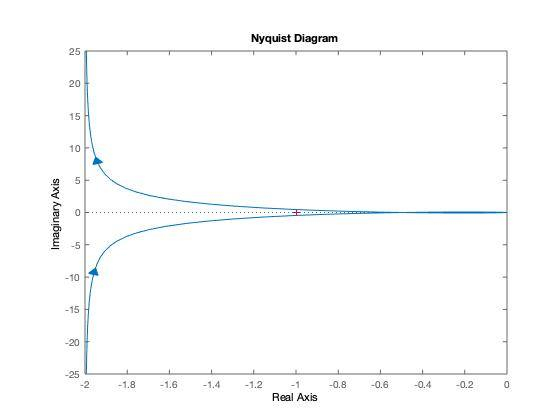
\includegraphics[width=0.8\textwidth]{./figures/lab8-Nyquist-Phase-Diagram.jpg}
	\caption{}
	\label{fig:}
\end{figure}

\begin{figure}[H]
	\centering
	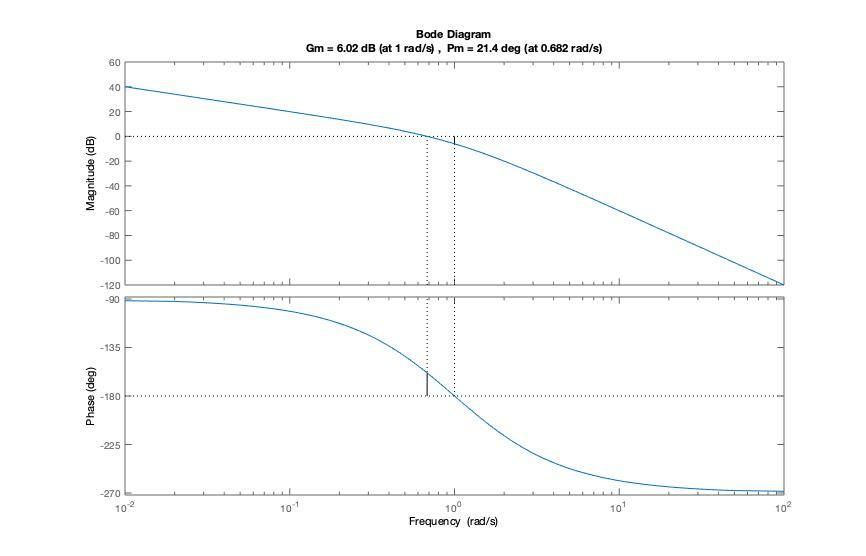
\includegraphics[width=0.8\textwidth]{./figures/lab8-Bode-Phase-Diagram.jpg}
	\caption{}
	\label{fig:}
\end{figure}
